\fbox{\parbox{\linewidth}{
        Vorliegendes Template enth\"alt exemplarisch (und damit unvollst\"andig) Gliederungspunkte, Bestandteile und Hinweise f\"ur ein typisches Softwareentwicklungsprojekt, bei dem ein Prototyp erstellt wird. Es dient als Hilfestellung zu Ihrer weiteren Verwendung. Selbstverst\"andlich m\"ussen Sie selbst weitere Erg\"anzungen und Anpassungen vornehmen.

        \begin{center}
            \textbf{Viel Erfolg sowie gutes Gelingen bei Ihrer Abschlussarbeit!}
        \end{center}
    }}
\\
\linebreak[4]
\linebreak[4]
Der Textteil beginnt hier und wird arabisch mit dieser Seite beginnend mit \frqq1\flqq{} arabisch nummeriert. Der Textteil gliedert sich in Kapitel und Unterkapitel. Soll jede Hierarchieebene benannt werden, dann ist folgende Terminologie  \"ublich:

\begin{itemize}
    \item 1. Hierarchieebene: Hauptkapitel
    \item 2. Hierarchieebene: Kapitel
    \item 3. Hierarchieebene: Unterkapitel
    \item 4. Hierarchieebene: Abschnitt
\end{itemize}

Der inhaltliche Aufbau einer Abschlussarbeit im Studiengang
\textit{Internationale Medieninformatik} h\"angt selbstverst\"andlich vom Thema und vom Inhalt ab. Abweichungen von der diesem Template zu Grunde liegenden Gliederungsstruktur sind immer m\"oglich, manchmal sogar zwingend notwendig. Stimmen Sie sich diesbez\"uglich immer mit Ihren Gutachter(inne)n ab.


Vergessen Sie niemals, all Ihre verwendeten Quellen anzugeben und korrekt zu zitieren\footnote{Erg\"anzende Informationen k\"onnen Sie auch in eine Fu"snote auslagern. Hier wird die Fu"snote dazu genutzt, um Ihnen bei Interesse am Thema Zitation vertiefende Quellen (z.B. \autocite{balzert2011} oder \autocite{franck2013}) anzubieten.}. Quellen k\"onnen manuell referenziert und im Quellenverzeichnis eingetragen werden. Erg\"anzend bieten viele Textverarbeitungsssteme auch ausgelagerte Quellenverwaltungsdateien und - systeme an,  \"uber die mittels entsprechender Befehle im Textteil zitiert werden kann\footnote{Wie Sie hoffentlich feststellen werden, erfolgt die Literaturverwaltung in diesem Template mittels einer *.bib-Datei (diese enth\"alt die verwendeten Quellen), welche die *.tex-Datei mittels Verwendung von biblatex und bibtex erg\"anzt.}.

Visualisieren Sie im Textteil angemessen, z.B. mittels Abbildungen und Tabellen. Vorliegendes Template enth"alt beispielhaft eingebundene Abbildungen und eine Tabelle (vgl. f.), welche der Steinlausforschung\footnote{Analog zu Straube (In: \autocite{pschy}) handelt es sich bei der Steinlaus (\textit{petrophaga lorioti}) um das \frqq \textit{kleinste einheimische Nagetier}\flqq. Als stimmungsaufhellender Endoparasit erreicht es eine Gr\"o"se von ca. 0,3 bis 3 mm und stammt aus der Familie der Lapivora. Die Steinlaus kommt ubiquit\"ar vor und ist in der Regel apathogen.} entnommen sind.


\begin{figure}
    \centering
    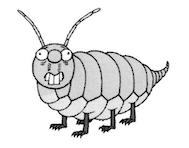
\includegraphics{images/steinlaus.jpg}
    \caption{Beispielgrafik: Steinlaus; Bildquelle \autocite{loriot}}
\end{figure}



\begin{figure}
    \centering
    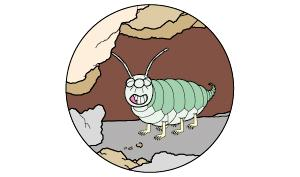
\includegraphics{images/steinlaus2.jpg}
    \caption{Beispielgrafik: Fressende Steinlaus; Bildquelle \autocite{loriot2}}
\end{figure}

\begin{table}
    \caption{\"Ubersicht: Untersuchte Steinl\"ause}
    \centering
    \begin{tabular}{llr}
        \toprule
        \multicolumn{2}{c}{Untersuchte Objekte mit Lokation des Habitats}           \\
        \cmidrule(r){1-2}
        ID (nickname)         & Ort                      & Gr\"o"se/L\"ange (in mm) \\
        \midrule
        1 (Rosalinde)         & Berlin, Mauerpark        & $1.4$                    \\
        2 (Devil in disguise) & Brandenburg, BER-Airport & $2.8$                    \\
        3 (Hannes)            & Berlin, Olympia-Stadion  & $2.1$                    \\
        4 (Her Majesty)       & Berlin, Humboldt-Forum   & $2.0$                    \\
        \bottomrule
    \end{tabular}
\end{table}

\section{Hintergrund der Arbeit}
 [Beschreibung des groben Kontextes der Arbeit; im Detail sollten Sie dies im Grundlagenteil darstellen]


\section{Problem- und Zielstellung (Scope)}
 [Beschreibung der Problemstellung sowie der sich daraus ergebenden Teilprobleme,-ziele und Forschungsfrage(n), welche Sie mit Ihrer Arbeit addressieren]


\section{Aufbau der Arbeit}
 [Beschreibung des Aufbaus der Arbeit]
